\documentclass[10pt,letterpaper]{article}

\usepackage{cvpr}
\usepackage{float}
\usepackage{amsmath}
\usepackage{amssymb}
\usepackage{caption}
\usepackage{booktabs}
\usepackage{graphicx}

\setcounter{figure}{3}
\setcounter{section}{6}
\definecolor{cvprblue}{rgb}{0,0,0}
\usepackage[pagebackref,breaklinks,colorlinks,allcolors=cvprblue]{hyperref}

\begin{document}

\section{Appendix}
\label{sec:appendix}

\begin{figure*}[htbp]
    \centering
    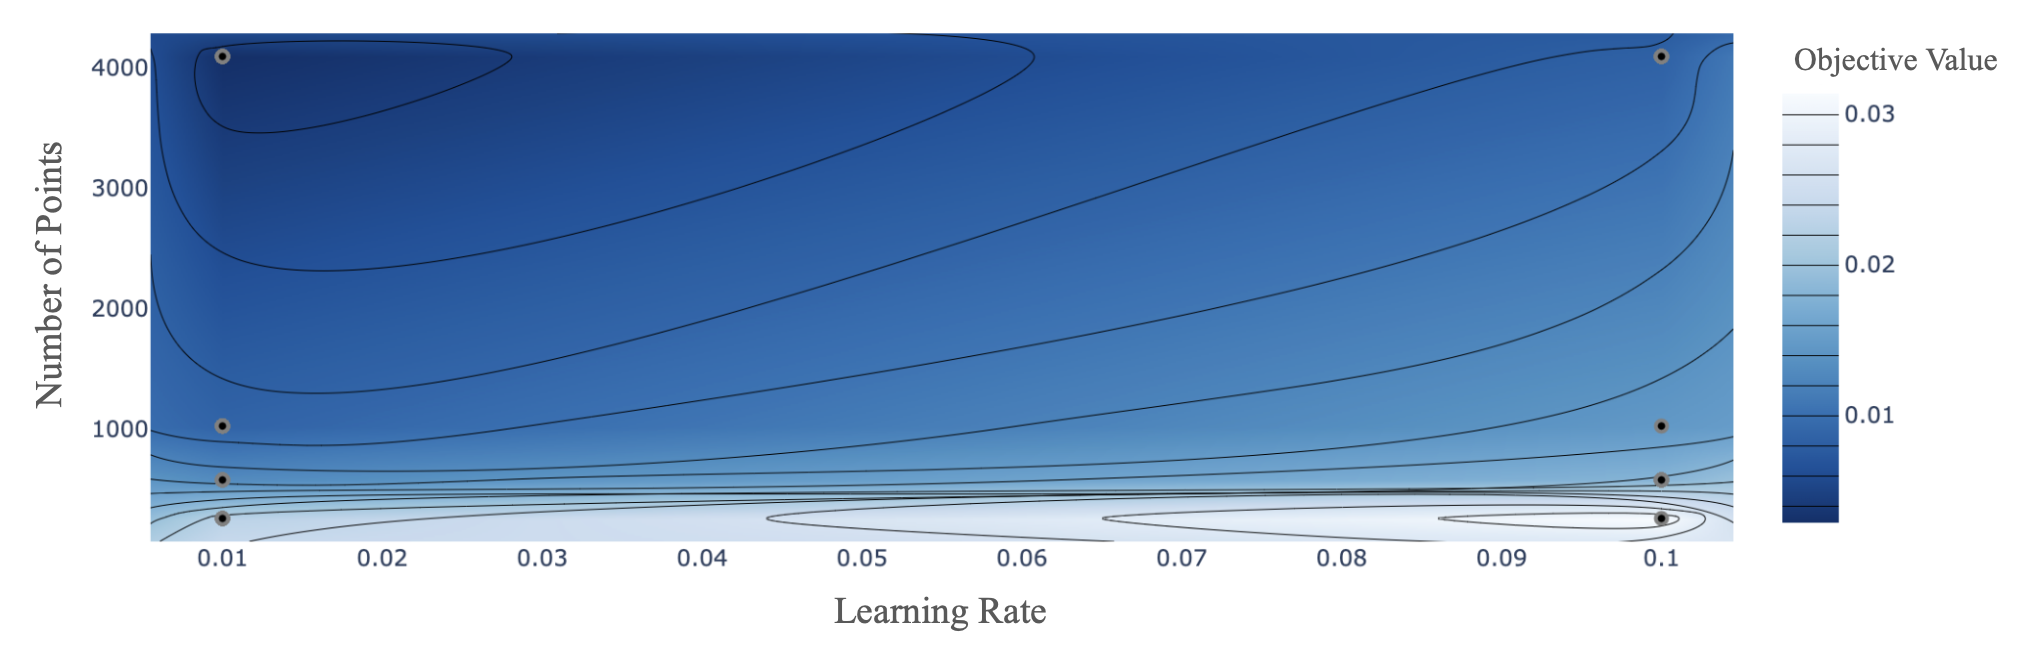
\includegraphics[width=1\linewidth]{fig/contour.png}
    \caption{\textbf{Contour Plot of Learning Rate and Number of Gaussian Primitives.} We identified the learning rate and the number of Gaussian primitives (points) as the two most decisive factors for the fidelity of Gaussian splat reconstructions. Clearly, a larger number of points results in higher reconstruction quality. Interestingly, the optimal learning rate for $1024$ points produces a comparable loss to a suboptimal learning rate even when using $4096$ points.}  
    \label{fig:contour}
\end{figure*}


\begin{figure*}[htbp]
    \centering
    \begin{subfigure}[b]{0.49\linewidth}
        \centering
        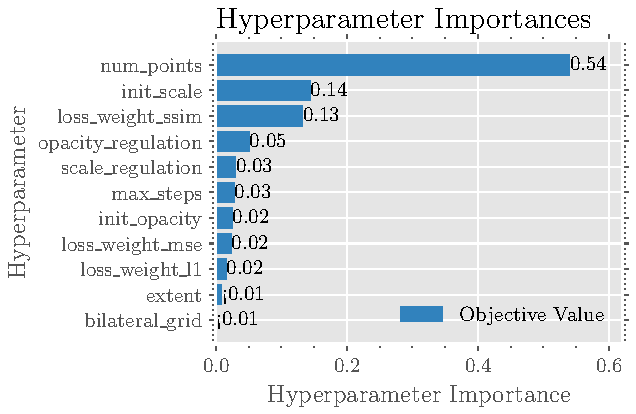
\includegraphics[width=\linewidth]{fig/splatting_param_importances_1.pdf}
        \caption{}
        \label{fig:splat-reconstructions-1}
    \end{subfigure}
    \hfill
    \begin{subfigure}[b]{0.49\linewidth}
        \centering
        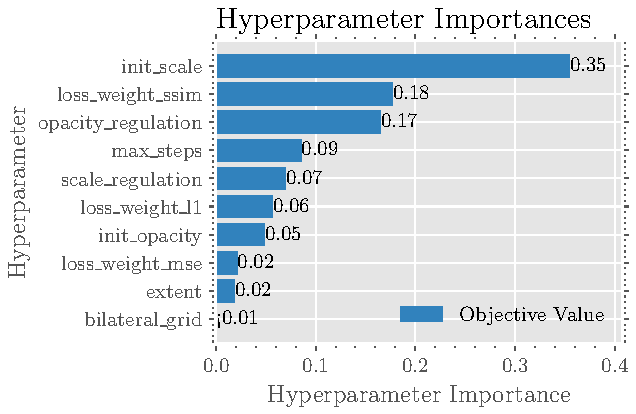
\includegraphics[width=\linewidth]{fig/splatting_param_importances_2.pdf}
        \caption{}
        \label{fig:splat-reconstructions-2}
    \end{subfigure}
    \caption{\textbf{Comparison of Hyperparameter Importance for Gaussian Splatting.} We evaluated the importance of each hyperparameter in learning Gaussian splats. The results indicate that the number of points is by far the most important parameter (\ref{fig:splat-reconstructions-1}), which is expected since more splats likely lead to better results. On the other hand, we also observe that initial scale and opacity, as well as their regularization, have a significant impact (\ref{fig:splat-reconstructions-2}).}
    \label{fig:splat-reconstructions-combined}
\end{figure*}

\begin{figure*}[htbp]
    \centering    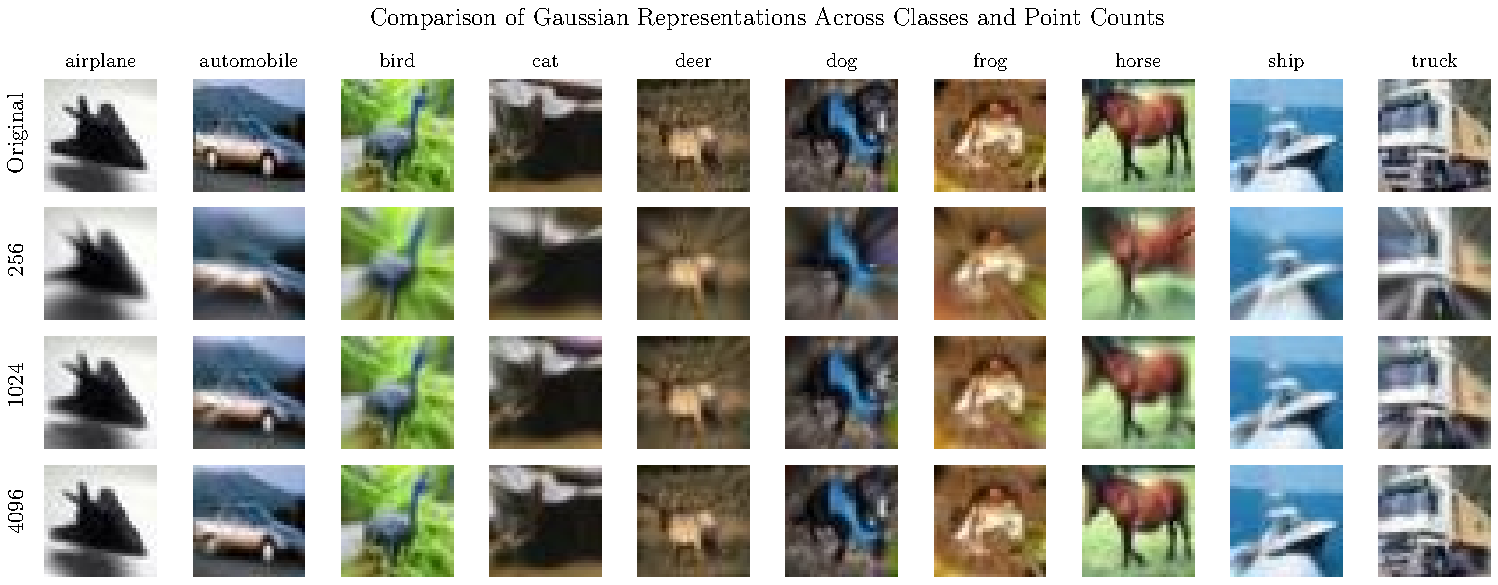
\includegraphics[width=1\linewidth]{fig/splatting_comparison_grid.pdf}
    \caption{\textbf{Gaussian Splat Reconstruction of CIFAR-10 Classes.} Example reconstructions for one image from each CIFAR-10 class. The top row shows the original images, while the middle and bottom rows display the Gaussian Splat reconstructions using grid- and KNN-initializations, respectively.}  
    \label{fig:splatting_comparison_grid}
\end{figure*}

\begin{figure*}[htbp]
    \centering    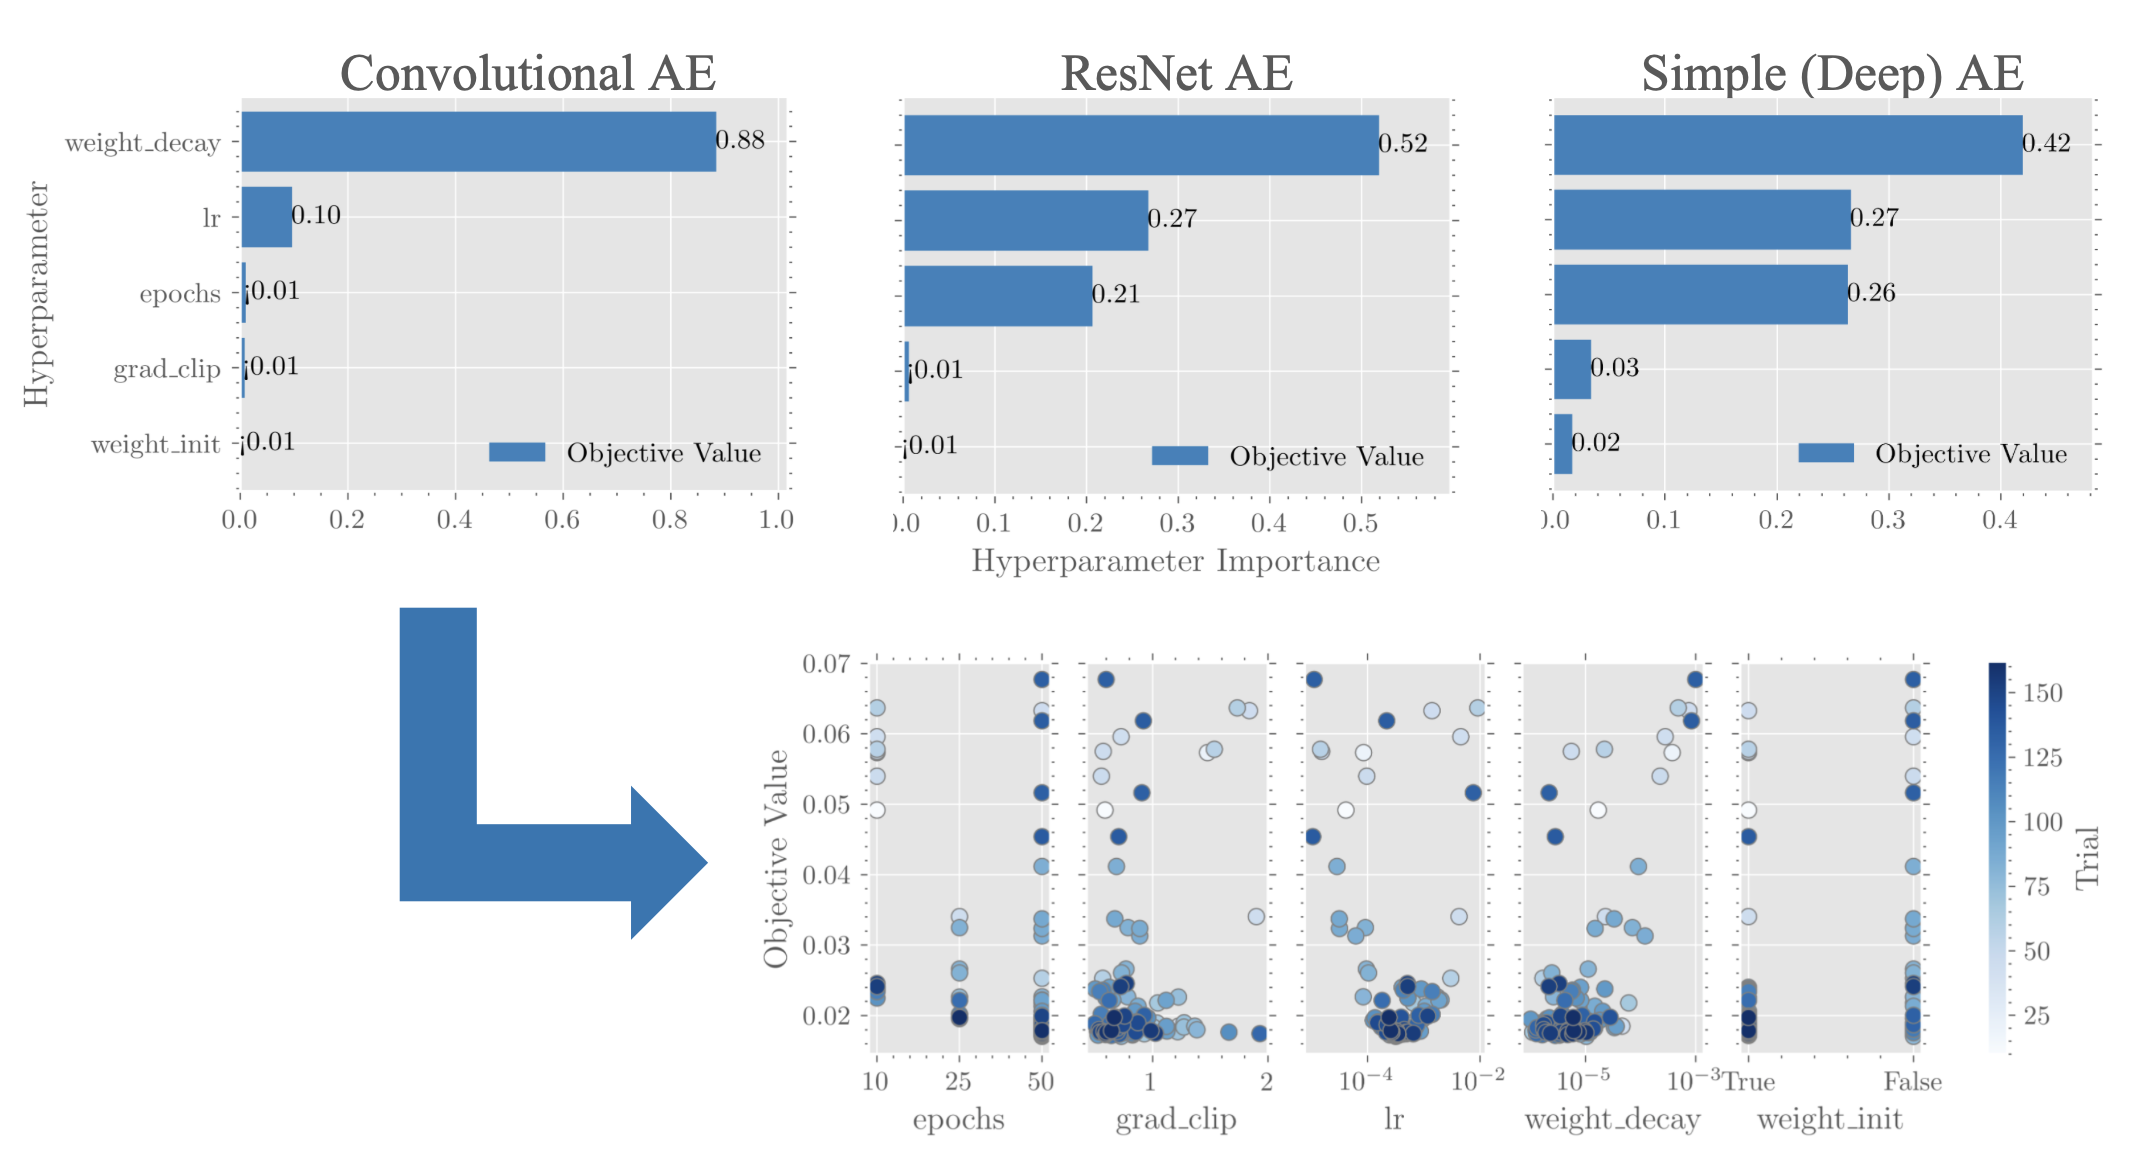
\includegraphics[width=1\linewidth]{fig/ae_hyperparam_tuning.png}
    \caption{\textbf{Comparison of Hyperparameter Importance for Autoencoding.} Comparison of the importance of different hyperparameters across the implemented AE architectures. We observe that weight decay and learning rate are the most important factors across all three approaches. The comparison below shows how the loss changes during optimization trials for different hyperparameter combinations in the convolutional AE.}
    \label{fig:splat-ae_hyperparam_tuning}
\end{figure*}

\begin{figure*}[htbp]
    \centering    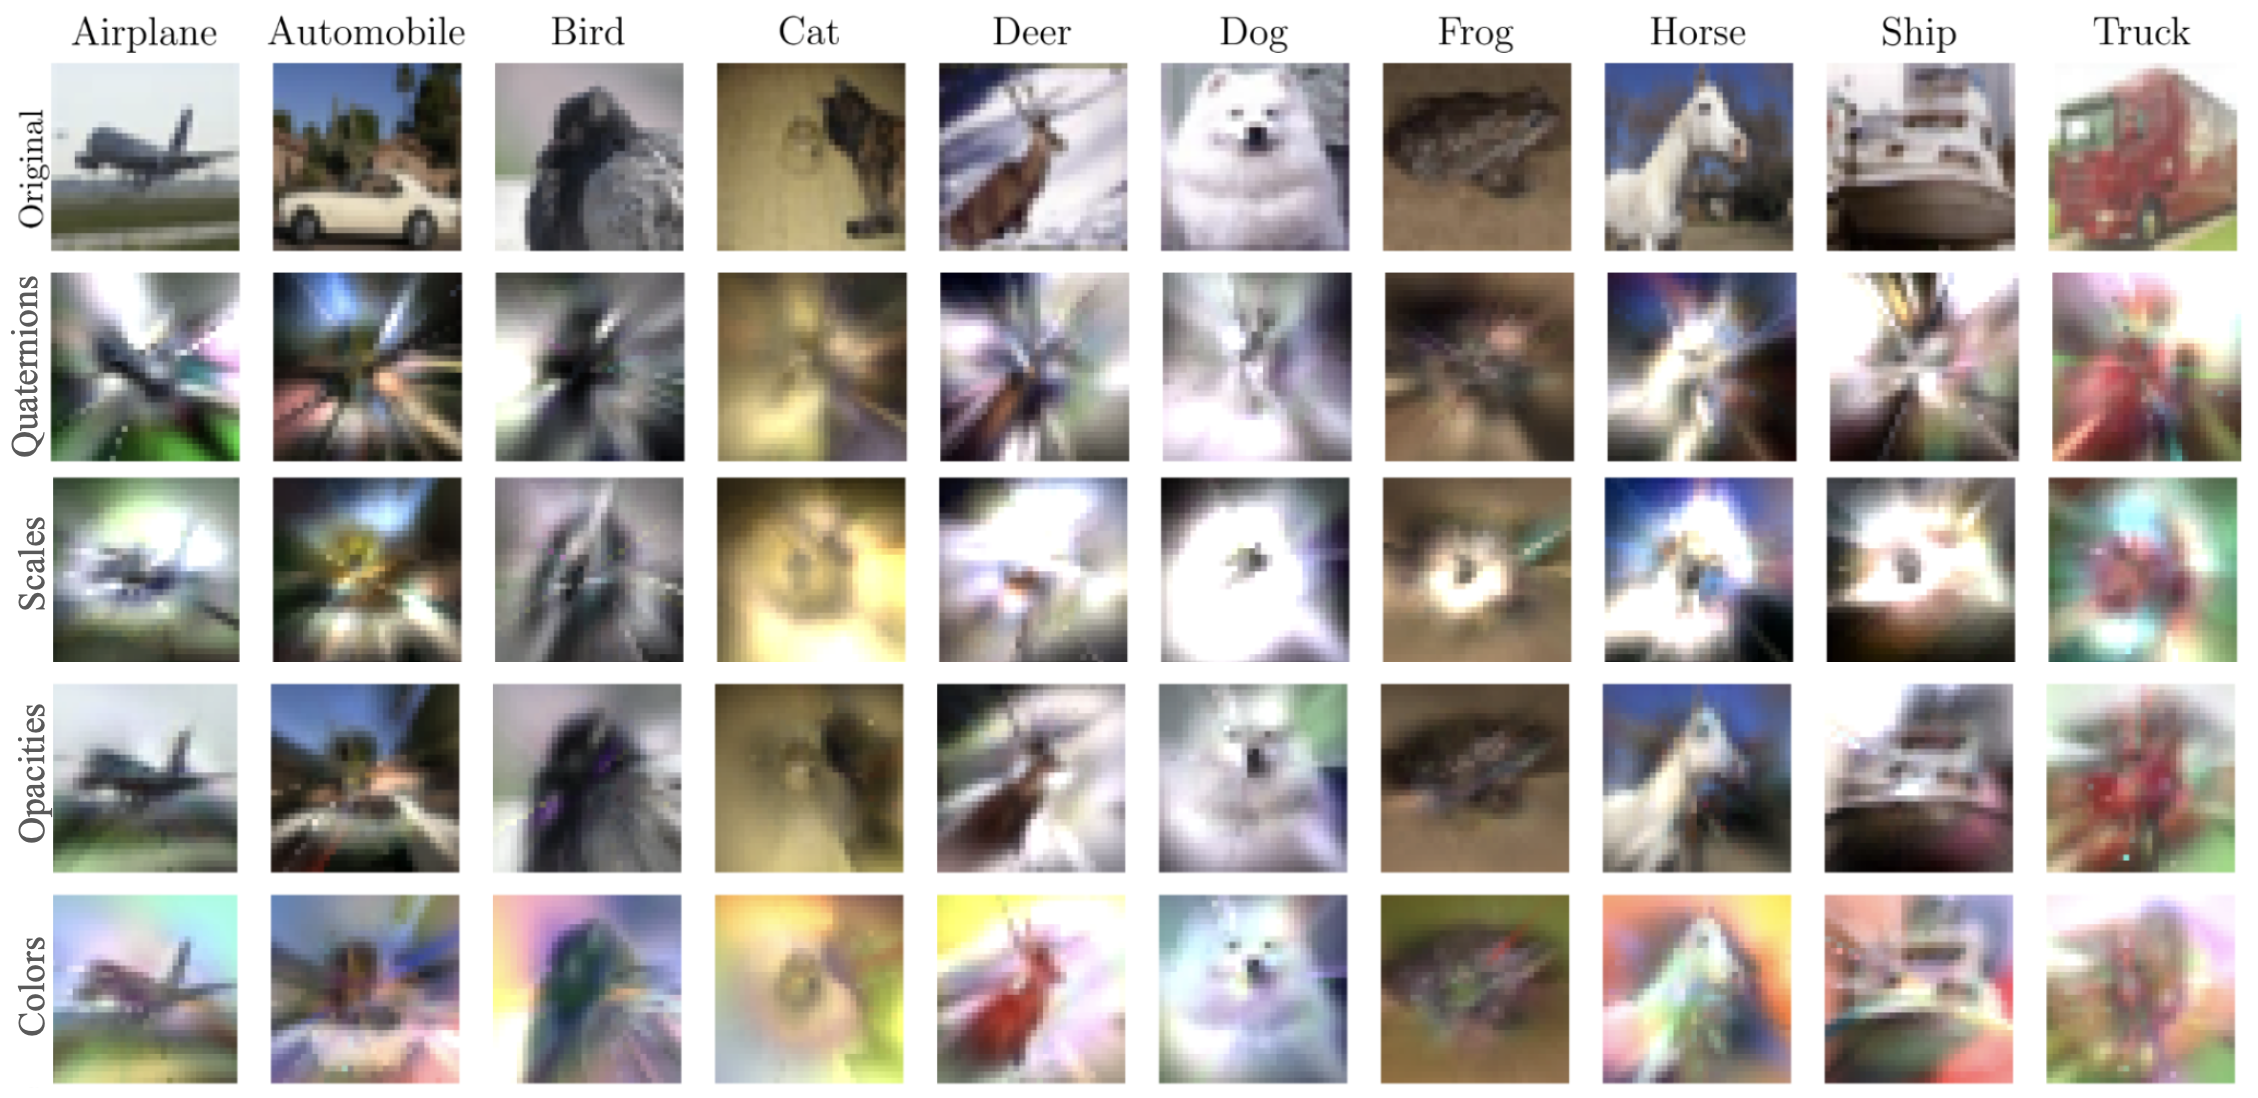
\includegraphics[width=1\linewidth]{fig/output_individual_params.png}
    \caption{\textbf{Comparison of Individual Autoencoded Splat Parameters.} Example reconstruction where only a single autoencoded Gaussian splat parameter is used to evaluate its impact on the image, while all other parameters are taken from the ground truth splat. The image shows that even small differences in the quaternion (rotation) parameter result in the most significant visual changes to the reconstructed image.}
    \label{fig:splat-output_individual_params}
\end{figure*}

\begin{figure*}[htbp]
    \centering    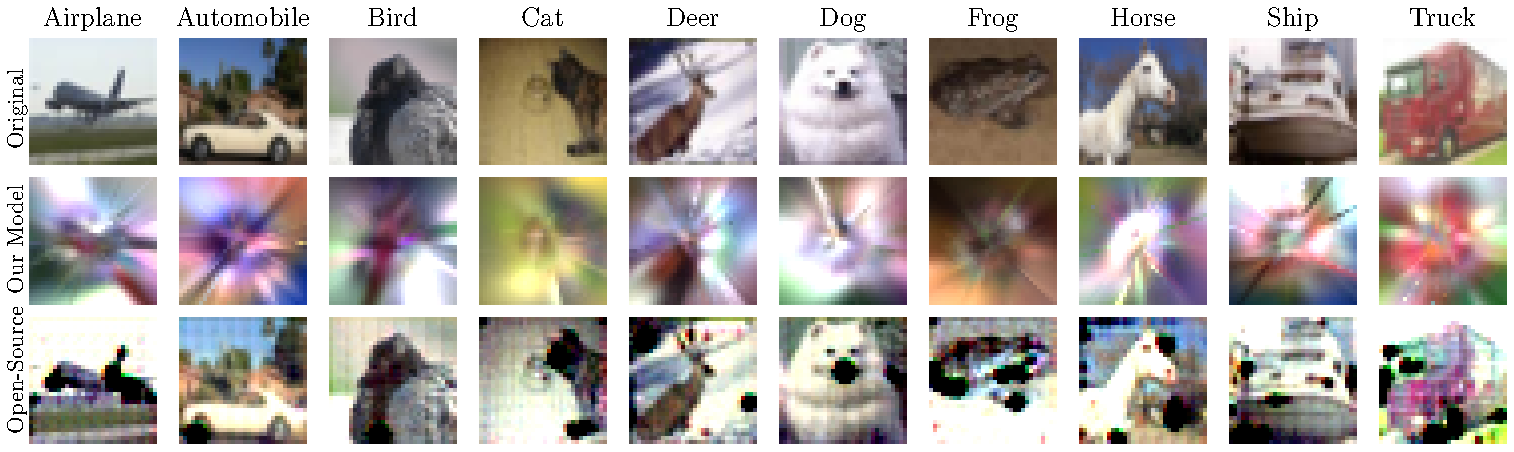
\includegraphics[width=1\linewidth]{fig/reconstruction_comparison_large_latent.pdf}
    \caption{\textbf{Reconstruction of Autoencoded Images and Gaussian Splats Using a Larger Latent Space.} This image is analogous to Fig. 3, but the images on the second row were autoencoded by a slightly different model variant. In this case, we used the Convolutional model again, but we removed a Max-Pooling layer and adapted the decoder to match it, resulting in a larger latent space ($8\times8$ instead of $4\times4$). Some of the resulting images have slightly more accurate colors, for instance the deer image, but in general the results are similar.}
    \label{fig:splat-output_individual_params}
\end{figure*}

\end{document}